\begin{frame}{Descripción del problema}
Considere un brazo robótico planar compuesto por dos eslabones de longitudes \(L_{1}\) y \(L_{2}\), articulados mediante ángulos \(\theta_{1}\) (el que forma el primer eslabón con la base de soporte) y \(\theta_{2}\) (el que forma el segundo eslabón respecto al primero).

\begin{figure}
    \centering
    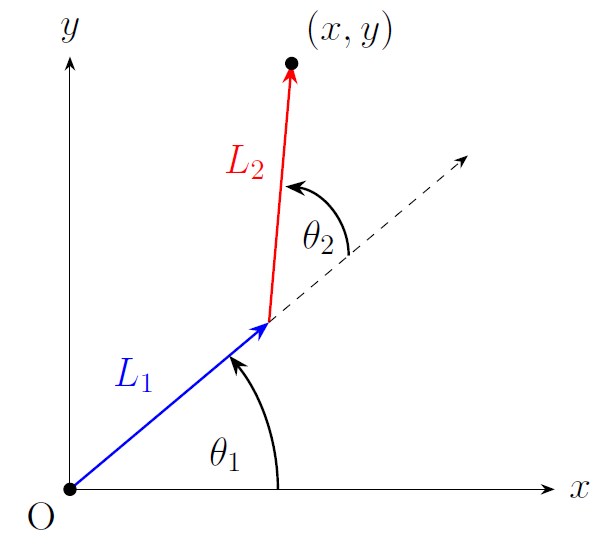
\includegraphics[width=0.35\linewidth]{graphics/grafica_descripcion.png}
\end{figure}  
\end{frame}

\begin{frame}{Descripción del problema}
La posición del extremo del brazo en el plano (en coordenadas cartesianas) está dada por:
\[
x(\theta_{1}, \theta_{2}) = L_{1}\cos(\theta_{1}) + L_{2}\cos(\theta_{1}+\theta_{2})
\]

\[
y(\theta_{1}, \theta_{2}) = L_{1}\sin(\theta_{1}) + L_{2}\sin(\theta_{1}+\theta_{2})
\]

Para alcanzar un punto deseado \((x_{d}, y_{d})\), se plantea el sistema no lineal:
\[
F_{1}(\theta_{1}, \theta_{2}) = x(\theta_{1}, \theta_{2}) - x_{d} = 0
\]
\[
F_{2}(\theta_{1}, \theta_{2}) = y(\theta_{1}, \theta_{2}) - y_{d} = 0
\]
\end{frame}
